\documentclass{csse4400}

\usepackage{tikz}
\usetikzlibrary{positioning}
\usetikzlibrary{arrows}

\usepackage{float}

\usepackage{enumitem}

\usepackage{languages}

\title{Codegram}
\author{Brae Webb}

\date{\week{2}}
\begin{document}

\maketitle


\section{Brief}

You are working on Codegram,
a social media website where programmers can post screenshots of their favourite code to share with others.
Naturally, developers want their code screenshots to look as good as possible,
so many users are requesting image filter features to make their screenshots look more appealing.

You have been tasked to design the backend for this feature.
The frontend team has developed the user interface.
Images are already uploaded and accessible via a URL that is provided to your backend.


\section{Requirements}

\begin{enumerate}
    \item The frontend should be able to make a HTTP request to the backend to apply a filter to an image.
    \item The HTTP request should include the URL of the image to be filtered.
    \item You can design the HTTP request however you like.
    \item The response should be the filtered image. You do not need to re-upload the image.
    \item The current filter options are:
          \begin{itemize}
              \item \textbf{Brightness}: Increase or decrease the brightness of the image.
              \item \textbf{Contrast}: Increase or decrease the contrast of the image.
              \item \textbf{Saturation}: Increase or decrease the saturation of the image.
              \item \textbf{Grayscale}: Converts the image to grayscale.
              \item \textbf{Sepia}: Converts the image to sepia.
              \item \textbf{Blur}: Blurs the image.
          \end{itemize}
          But you should expect more filters to be added in the future.
\end{enumerate}


\section{Outline}

\subsection*{Introduction (5 minutes)}
\begin{itemize}[topsep=5pt,partopsep=2pt,itemsep=2pt,parsep=2pt]
    \item Introduction to the brief.
    \item What is a filter.
    \item What are the requirements.
    \item Where to start.
\end{itemize}

\subsection*{Design (10 minutes)}
Individually, or in pairs, sketch out a potential design for the backend.
You can use any tools you like, but you should be able to explain your design to the class.
Your design does not need to be complete or perfect.
Try to be creative so that we can discuss the pros and cons of various design options.

\subsection*{Discussion (10 minutes)}
With the class, present a few of the designs and discuss the pros and cons of each.
Consider the following questions:
\begin{itemize}
    \item Does the design meet the requirements?
    \item Which quality attributes are prioritised in this design?
    \item How would you extend this design to support more filters?
    \item Are there trade-offs in this design?
\end{itemize}

\subsection*{Sketching (20 minutes)}
Individually sketch out a basic implementation of your preferred design from the discussion.
Your design sketch should include:
\begin{itemize}
    \item A high-level overview of the system, including any architectural patterns used.
    \item A description of the format of the HTTP request and response.
    \item An example of a HTTP request and response.
    \item A free-form diagram that illustrates the communication between components of the system.
\end{itemize}
You may include any other details including pseudocode, class diagrams, etc. that you think are relevant.

\subsection*{Optimisation (10 minutes)}
Discuss how you would optimise your design to improve extensibility, performance, scalability, etc. in a real system.
Consider the following questions:
\begin{itemize}
    \item What are the time/computation consuming parts of your design?
    \item Are there any bottlenecks?
    \item Are there use cases of the system that you can optimise? e.g. What if users repost and filter the same image?
    \item How would you scale your design to support more users?
    \item Are there any security concerns?
\end{itemize}


\section{Design Challenges}

\subsection*{Challenge 1: Malicious Images}
Codegram routinely scans hashes of uploaded images to detect malicious images, such as uploads of PHP code.
Users have used the filter feature to bypass this detection.
How would you modify your design to prevent this?

\subsection*{Challenge 2: Reordering Filters}
Codegram users often apply the same filter in different orders.
For example, they may apply the \texttt{grayscale} filter then the \texttt{brightness} filter,
or the \texttt{brightness} filter then the \texttt{grayscale} filter.
How would you optimise your design to reduce the number of times the image is filtered?
Could you conceive of filters that are not commutative (i.e. the order matters)?

\subsection*{Challenge 3: Global Access}
Codegram is a global service, and users are located all over the world.
Some users have reported that the filter feature is slow.
You have determined that the primary cause is the latency between the user and the server.
How would you modify your design to reduce the latency?


\section{Programming Challenge}
In a programming language of your choice,
attempt a basic implementation of your preferred design.
Use any libraries you like to implement the image filters, e.g. Pillow, OpenCV, etc.
You do not need to implement the HTTP request, you can simulate it by calling a function in your code,
but creating Web APIs will be important in the course so this is good practice.
Refer to the week 1 practical \cite{prac-week1} for an example of how to create a Web API.


\bibliographystyle{ieeetr}
\bibliography{ours}

\end{document}


% TODO(bw): Move case studies into handout
\section{Case Study: Compilers}

An interesting case study of the pipeline architecture is a compiler.%
\footnote{You do not need to understand the phases of a compiler --- two data structures, the Symbol Table and Abstract Syntax Tree (AST), are transformed in each compiler phase.}
As a foundational technology, compilers have undergone rigorous refinement and are perhaps the most well studied type of software.
Modern compilers have well-defined modular phases as illustrated by Figure \ref{fig:compiler-architecture},
each phase of a compiler transforms the representation of the program until the target program is produced.

\begin{figure}[H]
    \centering
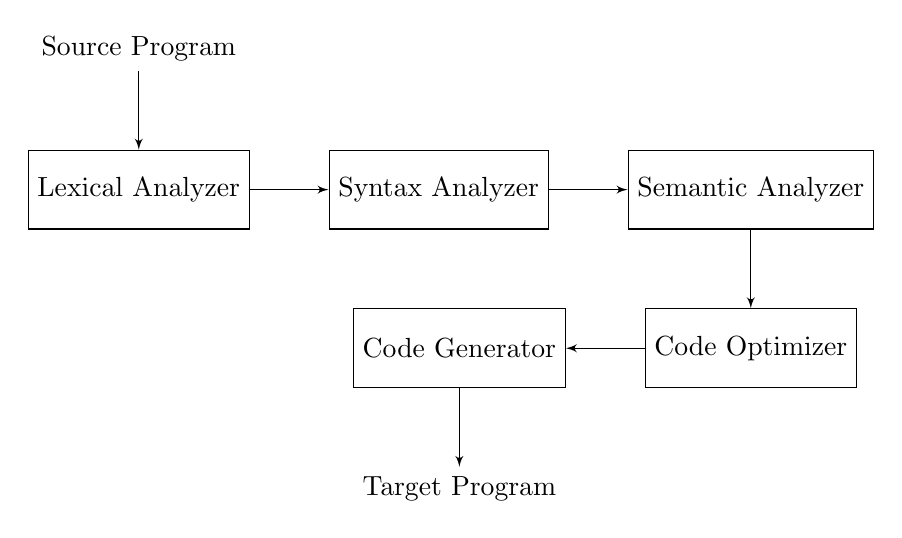
\begin{tikzpicture}[>=latex']
    \tikzset{block/.style= {draw, rectangle, align=center,minimum width=2cm,minimum height=1cm},}

    \node (src) {Source Program};
    \node [block, below =1cm of src] (lex) {Lexical Analyzer};
    \node [block, right =1cm of lex] (syn) {Syntax Analyzer};
    \node [block, right =1cm of syn] (sem) {Semantic Analyzer};
    \node [block, below =1cm of sem] (opt) {Code Optimizer};
    \node [block, left =1cm of opt] (gen) {Code Generator};
    \node [below =1cm of gen] (tar) {Target Program};

    \path[draw,->]
                (src) edge (lex)
                (lex) edge (syn)
                (syn) edge (sem)
                (sem) edge (opt)
                (opt) edge (gen)
                (gen) edge (tar)
                ;
\end{tikzpicture}
\caption{Typical phases of a compiler.}
\label{fig:compiler-architecture}
\end{figure}

However, a compiler is not well suited to use a pipeline architecture.
In general, the modules of a pipeline architecture should be independent of their input source.
This is not the case in compilers, as each phase relies on the completion of the previous phase.
As a result, the input dependencies of a compiler make it too restrictive for a true pipeline architecture.

Instead, compilers are often built as a hybrid of a pipeline architecture and the \textsl{Blackboard Architecture}.
The blackboard architecture consists of;
\begin{itemize}
    \item a knowledge base, the `blackboard',
    \item knowledge sources which use and update the knowledge base, and
    \item a control component to coordinate the operation of knowledge sources.
\end{itemize}

In modern compilers, the data which would be passed through pipes, the Symbol Table and AST,
are used and updated by each phase.
They are subsequently used as the `blackboard'.
Each phase is considered a knowledge source which uses the knowledge base to transform and update the knowledge base.
Finally, in this hybrid, the control component is not required as the sequence of phase execution in a pipeline coordinates operation.
Figure \ref{fig:compiler-architecture-sym} illustrates this proposed architecture.
Of course, there are many compilers out there, many of them deviate from this architectural hybrid.

\begin{figure}[H]
    \centering
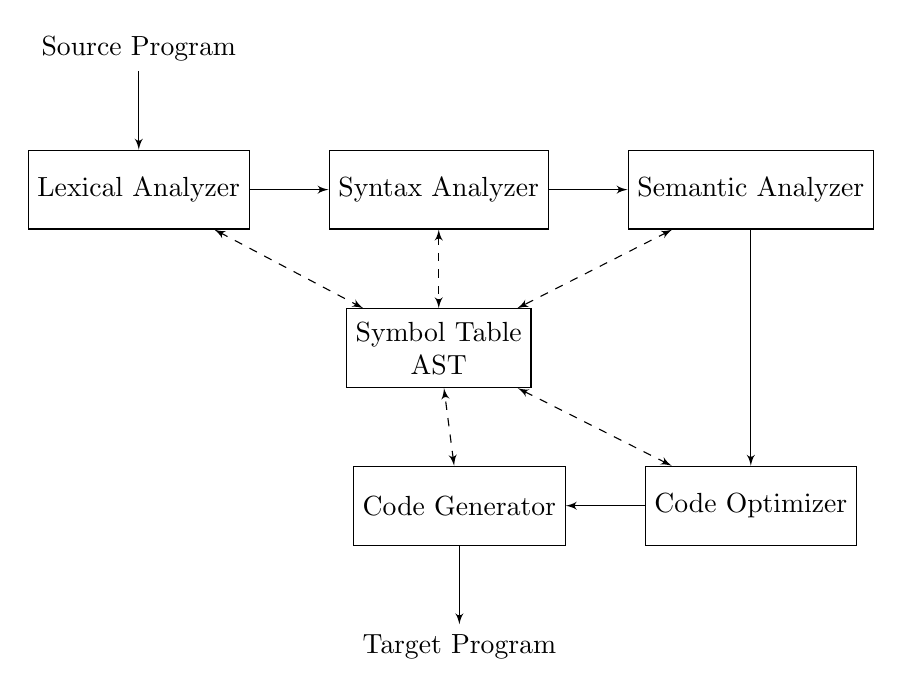
\begin{tikzpicture}[>=latex']
    \tikzset{block/.style= {draw, rectangle, align=center,minimum width=2cm,minimum height=1cm},}

    \node (src) {Source Program};
    \node [block, below =1cm of src] (lex) {Lexical Analyzer};
    \node [block, right =1cm of lex] (syn) {Syntax Analyzer};
    \node [block, right =1cm of syn] (sem) {Semantic Analyzer};
    \node [block, below =3cm of sem] (opt) {Code Optimizer};
    \node [block, left =1cm of opt] (gen) {Code Generator};
    \node [below =1cm of gen] (tar) {Target Program};

    \node [block, below =1cm of syn] (sym) {Symbol Table\\AST};

    \path[draw,->]
                (src) edge (lex)
                (lex) edge (syn)
                (syn) edge (sem)
                (sem) edge (opt)
                (opt) edge (gen)
                (gen) edge (tar)
                ;

    \path[draw,<->,dashed] (lex) edge (sym);
    \path[draw,<->,dashed] (syn) edge (sym);
    \path[draw,<->,dashed] (sem) edge (sym);
    \path[draw,<->,dashed] (opt) edge (sym);
    \path[draw,<->,dashed] (gen) edge (sym);
\end{tikzpicture}
\caption{Phases of a modern compiler.}
\label{fig:compiler-architecture-sym}
\end{figure}

\section{Case Study: MapReduce}

One of the more prevalent uses of the pipeline architecture is the MapReduce pattern.
The MapReduce pattern was discovered in 2004 as a solution to the challenges which Google faced managing their search index \cite{mapreduce}.%
\footnote{Although the pattern was in use prior to their work\cite{mapreduce-critique}} %
MapReduce affords impressive parallelism inherit to the programming pattern.

The two key ideas of MapReduce, are \textsl{map} and \textsl{reduce}.
Below are the generic types of the \textsl{map} and \textsl{reduce} functions in functional programming.

\begin{code}[language=lambda]{}
map : (type$_1$ -> type$_2$) -> type$_1 Seq$ -> type$_2 Seq$
map $f$ $xs$
reduce : (type$_2$ -> type$_1$ -> type$_2$) -> type$_1 Seq$ -> type$_2$ -> type$_2$
reduce $f$ $xs$ $initial$
\end{code}

If you are unfamiliar with this notation, the rough English translation is:
\begin{description}
    \item[map] The parameters of the \textsl{map} function are:
        \begin{enumerate}[label=(\alph*)]
            \item A function, $f$, which takes a parameter of type $\tau_1$ and returns a type $\tau_2$.
            \item A sequence of elements of type $\tau_1$.
        \end{enumerate}
        The return type of the \textsl{map} function is a sequence of elements of type $\tau_2$.
    \item[reduce] The parameters of the \textsl{reduce} function are:
        \begin{enumerate}[label=(\alph*)]
            \item A function, $f$, which takes two parameters, the first of type $\tau_2$ is the current accumulator value, the second of type $\tau_1$ is the current value in the input sequence, and returns a $\tau_2$, the new accumulator value.
            \item A sequence of elements of type $\tau_1$.
            \item An initial accumulator value of type $\tau_2$
        \end{enumerate}
        The return type of the \textsl{reduce} function is the type $\tau_2$.
\end{description}

The code snippet below uses the $map$ and $reduce$ functions
to perform the operations of the above bash example.
One important thing to note about the example below is the map operation on line 11.
Each application of the lambda function within the map operation is completely independent and could,
in theory, be executed simultaneously. 

\begin{code}[language=python,literate={{->}{{$\to$}}{2}{lambda}{{$\lambda$}}{1}},morekeywords={then}]{}
contents = read("assignment.py")

# filter relevant lines by rebuilding the list
contents = reduce(lambda xs x -> 
                      if x.contains("hack")
                        then x + xs
                        else xs,
                    contents,
                    [])

# use map to count occurrences of word
contents = map(lambda line -> line.count("hack"), contents)

# use reduce to sum list of counts
contents = reduce(lambda total curr -> total + curr, contents, 0)

write("code-quality.txt", contents)
\end{code}

So by design, code written in this pattern can process data simultaneously.
Tools such as \link{Hadoop}{https://hadoop.apache.org/} are able to take advantage of this to distribute computation automatically.

\begin{extra}
Using the terminology of a pipeline architecture, what filters do the \textsl{map} and \textsl{reduce} operators roughly correspond to?
\end{extra}

\begin{extra}
How would you improve the efficiency of the code snippet above?
\end{extra}

\bibliography{articles}

